\documentclass[slidestop, mathserif]{beamer}

% \mode<presentation>
% {
% 	\usetheme{Warsaw}
% 	\setbeamercovered{transparent}
% }

\mode<presentation>{
	\usetheme{Berlin}
	\setbeamercovered{transparent}
	\usefonttheme{professionalfonts}
}

\usepackage{amsmath, amsfonts, amssymb}

\newcommand{\norm}[1]{\left\|#1\right\|}

\AtBeginSection[]
{
   \begin{frame}
       \tableofcontents[currentsection]
   \end{frame}
}

%% want to use verbatim: \begin{frame}[fragile]

\title[Metrics for Tracking]{Metrics for Trackings: Evaluations and Comparisons}
\author[chy1010]{Chien, Hung-Yu (chy1010) \\ {\tt andy1010@gmail.com}}
\date{\today}

\begin{document}

\begin{frame}
    \titlepage
\end{frame}

% \section[Outline]{}
% \begin{frame}
%     \frametitle{Outlines}
%     \tableofcontents
% \end{frame}

\section{Preliminaries}

\begin{frame}
	\frametitle{MOT (Multiple Object Tracking)}

	Given a video, the task of MOT consists of the following parts:
	\begin{itemize}
		\item locating multiple objects,
		\item maintaining their identities, and
		\item yielding their individual trajectories.
	\end{itemize}

    In more details, each object is assigned a unique id in a frame.
    And objects with the same id in consecutive frames form a trajectory.

    \begin{figure}
        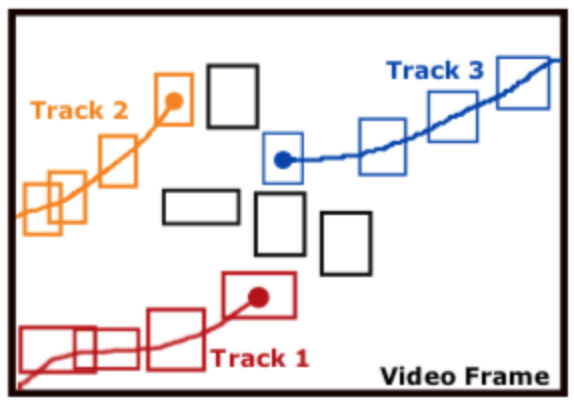
\includegraphics[height=70pt]{pics/fig1.png}
        \caption{objects with the same id from different frames}
    \end{figure}

\end{frame}

\begin{frame}
    \frametitle{Matching in Frame-Level}

    Here a {\bf matching} is a \emph{1-1 relation} between ground-truths
    and predictions.
    It can be done by according to the {\bf similarity scores} of every `gt-pred' pair.
    For example, $\max\{1-\text{\tt dist}, 0\}$ and {\tt IoU} are common metrics for measuring
    similarity, which is in $[0,1]$.

    \quad

    Denote $\mathcal S(g_i, p_j)$ be the similarity score of $i$-th ground-truth object
    and $j$-th prediction. Let $\alpha\in(0,1)$.
    Then a matching $\Pi$ under the similarity threshold $\alpha$ is a 1-1 relation satisfying
    \[
        (g,p) \in \Pi \Rightarrow \mathcal S(g, p) \geq \alpha.
    \]

    \vspace{5pt}

    \emph{1-1 relation: if $(g_i, p_j)$, $(g_k, p_\ell)\in \Pi$,
    then $i=k$ $\Leftrightarrow$ $j=\ell$.}

\end{frame}

\begin{frame}
    \frametitle{TP, FP and FN}

    For a given matching during all frames, we can define:
    \begin{itemize} \itemsep = 2pt
    \item TP (true positive cases): Matched pairs in a matching.
    \item FP (false positive cases): Non-matched predictions.
    \item FN (false negative cases): Non-matched ground-truth objects.
    \end{itemize}

    \begin{figure}
        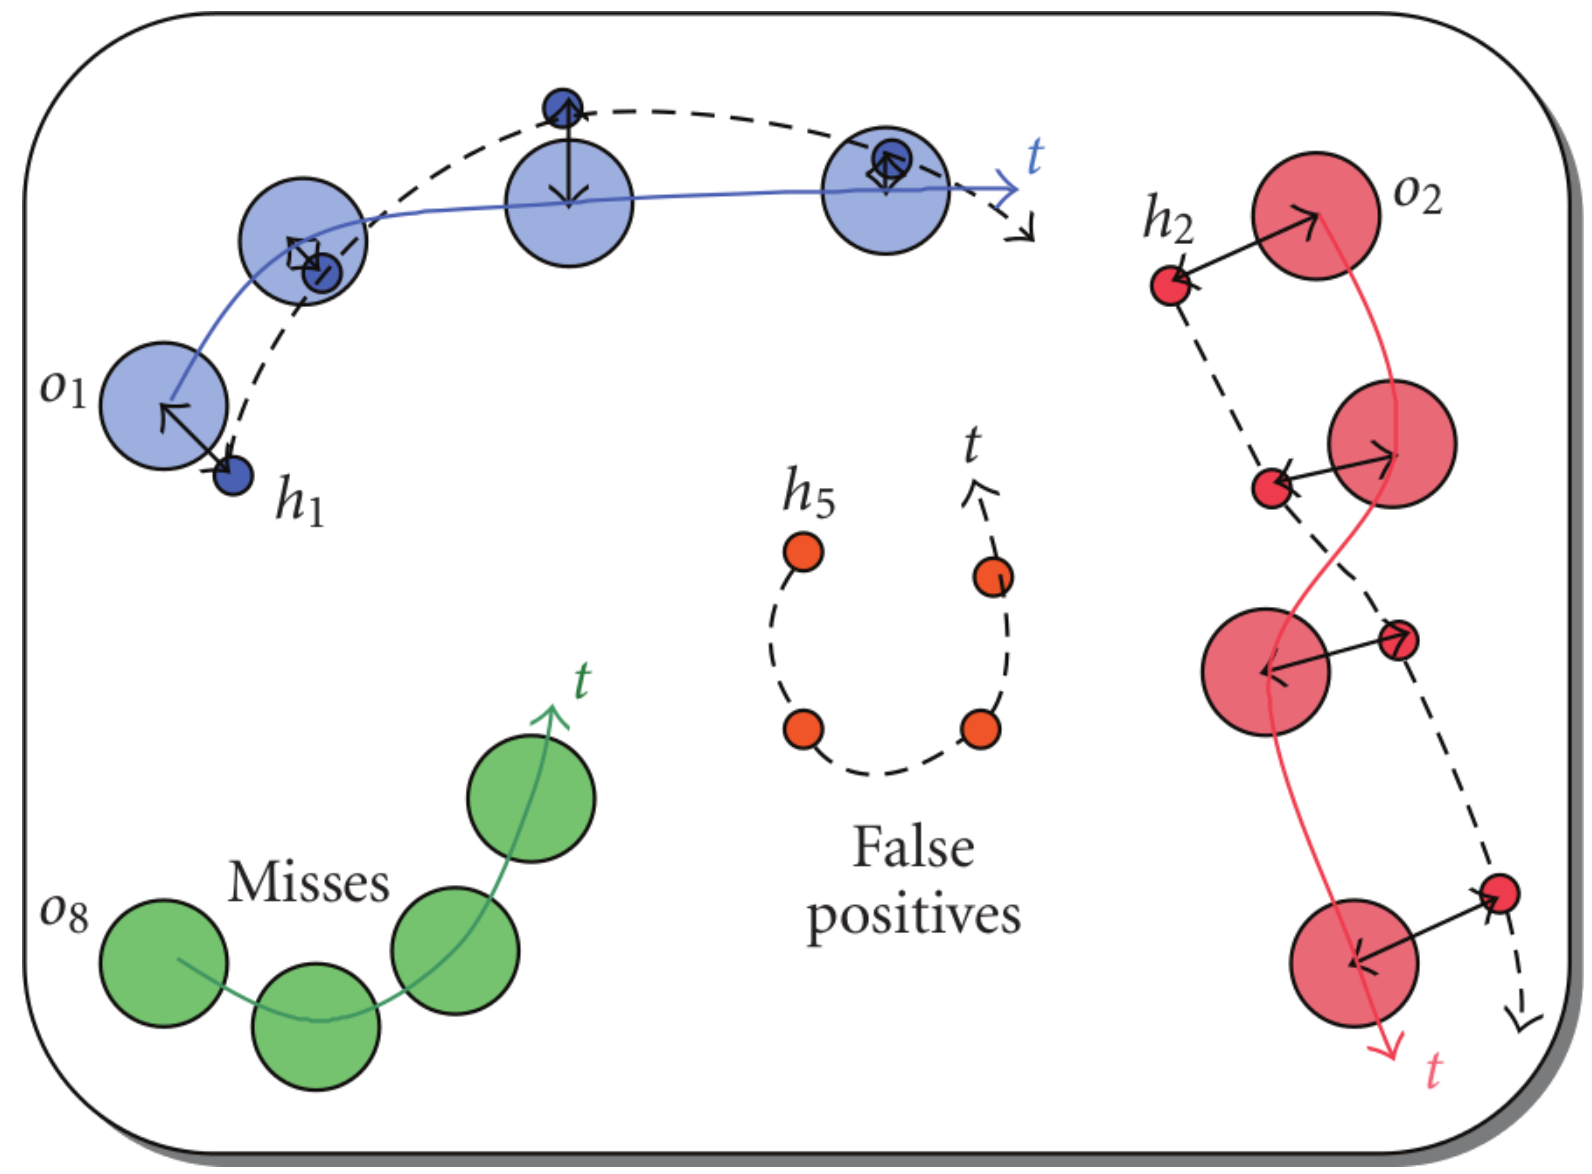
\includegraphics[height=90pt]{pics/fig2.png}
        \caption{TPs, FPs, FNs in consecutive frames.}
    \end{figure}

\end{frame}

\begin{frame}
    \frametitle{IDSW}

    An {\bf id switch} (IDSW) event means there exist $(g_i, p_j)\in\Pi^{(f)}$,
    $(g_k, p_\ell)\in\Pi^{(f+1)}$ TP pairs in two consecutive frames
    $f$ and $f+1$ that satisfy
    \[
        \text{gtId}(g_i) = \text{gtId}(g_k),\ 
        \text{prId}(p_j) \neq \text{gtId}(p_\ell).
    \]

    

\end{frame}

\begin{frame}
    \frametitle{Matching in Sequence-Level}

    
\end{frame}





\end{document}